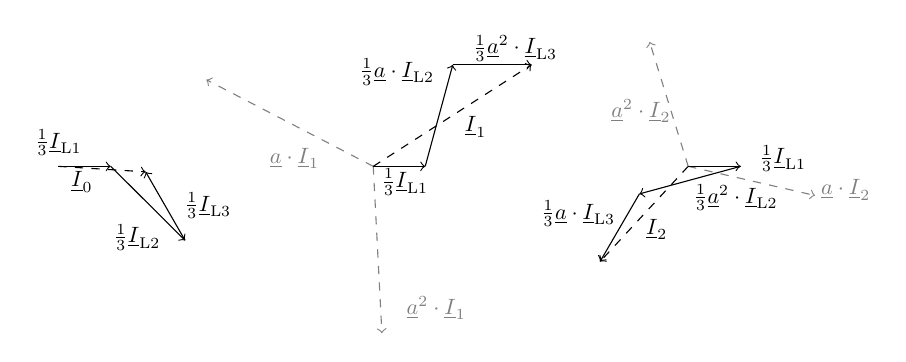
\begin{tikzpicture}
    \draw [->] [dashed] (0, -6) -- (2.01, -4.71);
    \draw [->, gray] [dashed] (0, -6) -- (-2.12, -4.9);
    \draw [->, gray] [dashed] (0, -6) -- (0.11, -8.12);
    \draw [->] (0, -6) -- (0.66, -6);
    \draw [->] (0.66, -6) -- (1.01, -4.71);
    \draw [->] (1.01, -4.71) -- (2.01, -4.71);

    \draw (1.3, -5.5) node [scale=0.8] {$\underline{I}_{\mathrm{1}}$};
    \draw (-1, -5.9) node [scale=0.8, gray] {$\underline{a}\cdot\underline{I}_{\mathrm{1}}$};
    \draw (0.8, -7.8) node [scale=0.8, gray] {$\underline{a}^2\cdot\underline{I}_{\mathrm{1}}$};
    \draw (0.4, -6.2) node [scale=0.8] {$\frac{1}{3}\underline{I}_{\mathrm{L1}}$};
    \draw (1.8, -4.5) node [scale=0.8] {$\frac{1}{3}\underline{a}^2\cdot\underline{I}_{\mathrm{L3}}$};
    \draw (0.3, -4.8) node [scale=0.8] {$\frac{1}{3}\underline{a}\cdot\underline{I}_{\mathrm{L2}}$};

    \draw [->] [dashed] (4, -6) -- (2.88, -7.21);
    \draw [->, gray] [dashed] (4, -6) -- (5.61, -6.37);
    \draw [->, gray] [dashed] (4, -6) -- (3.51, -4.42);
    \draw [->] (4, -6) -- (4.666, -6);
    \draw [->] (4.666, -6) -- (3.38, -6.35);
    \draw [->] (3.38, -6.35) -- (2.88, -7.21);

    \draw (3.6, -6.8) node [scale=0.8] {$\underline{I}_{\mathrm{2}}$};
    \draw (6, -6.3) node [scale=0.8, gray] {$\underline{a}\cdot\underline{I}_{\mathrm{2}}$};
    \draw (3.4, -5.3) node [scale=0.8, gray] {$\underline{a}^2\cdot\underline{I}_{\mathrm{2}}$};
    \draw (5.2, -5.9) node [scale=0.8] {$\frac{1}{3}\underline{I}_{\mathrm{L1}}$};
    \draw (4.6, -6.4) node [scale=0.8] {$\frac{1}{3}\underline{a}^2\cdot\underline{I}_{\mathrm{L2}}$};
    \draw (2.6, -6.6) node [scale=0.8] {$\frac{1}{3}\underline{a}\cdot\underline{I}_{\mathrm{L3}}$};

    \draw [->] [dashed] (-4, -6) -- (-2.89, -6.07);
    \draw [->] (-4, -6) -- (-3.334, -6);
    \draw [->] (-3.334, -6) -- (-2.39, -6.94);
    \draw [->] (-2.39, -6.94) -- (-2.89, -6.07);

    \draw (-3.7, -6.2) node [scale=0.8] {$\underline{I}_{\mathrm{0}}$};
    \draw (-4, -5.7) node [scale=0.8] {$\frac{1}{3}\underline{I}_{\mathrm{L1}}$};
    \draw (-3, -6.9) node [scale=0.8] {$\frac{1}{3}\underline{I}_{\mathrm{L2}}$};
    \draw (-2.1, -6.5) node [scale=0.8] {$\frac{1}{3}\underline{I}_{\mathrm{L3}}$};
\end{tikzpicture}